\section{CNN}

During the last years, time series classification has become one of the most challenging problems in Data Science. This has happened because any classification problem that uses data keeping in consideration some notion of sorting, can be treated as a time Series


In this section, we will review the neural networks especially deep learning methods for time series classification. 
Almost all machine learning algorithms, apart from those based on deep learning, require feature engineering process. These process can cause some information to be loss by expert mistake. On the contrary, deep learning models already incorporate this kind of feature engineering internally, optimizing it and eliminating the need to do it manually. Therefore they are able to extract information from the time series in a faster, more direct, and more complete way.





Generally, deep learning for time series classification fall into two types, CNN and RNN.

Another popular type of architectures for deep learning models is the RNN. Apart from time series forecasting, we found that these neural networks were rarely applied for time series classification which is mainly due to three factors: (1) the type
of this architecture is designed mainly to predict an output for each element (timestamp) in the time series (Längkvist, Karlsson, and Loutfi, 2014); (2) RNNs typically suffer from the vanishing gradient problem due to training on long time series (Pascanu, Mikolov, and Bengio, 2012); (3) RNNs are considered hard to train
and parallelize which led the researchers to avoid using them for computational reasons (Pascanu, Mikolov, and Bengio, 2013).


\paragraph{Functionality} The Elsevier article class is based on the standard article class and supports almost all of the functionality of that class. In addition, it features commands and options to format the
\begin{itemize}%\begin{enumerate}[(1)]
\item document style
\item baselineskip
\end{itemize}



\begin{figure}
    \centering
    \begin{minipage}[b]{.5\textwidth}
        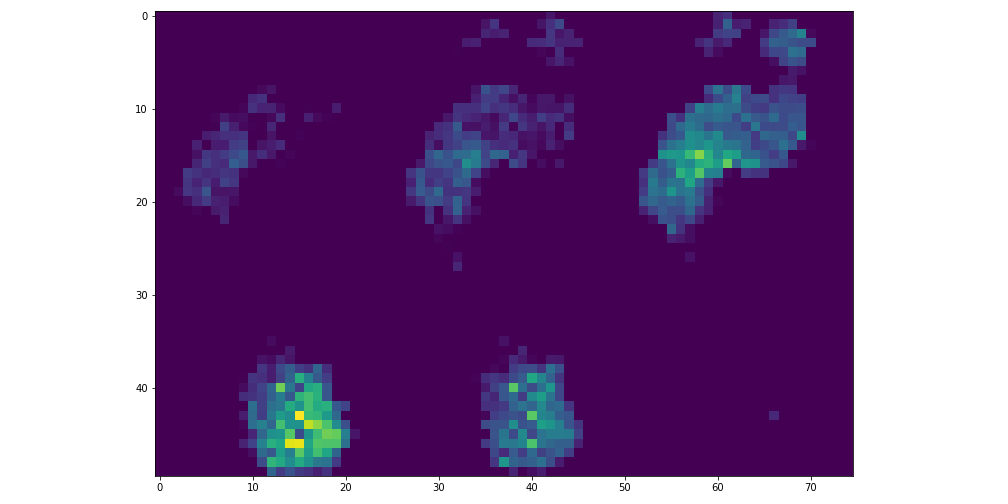
\includegraphics[width=\textwidth]{figures/project/frame1.png}
    \end{minipage}
    \caption{sample image.}
    \label{fig:Stepscan_dataset}
\end{figure}


Here are two sample references: \cite{SKazemii/EE6563}.